\documentclass{beamer}
\usetheme{Madrid}
\usepackage[french]{babel}
\usepackage[utf8]{inputenc}
\usepackage{graphicx}
\usepackage{hyperref}

\title{Projet Python -- Les Aventuriers du Rail}
\author{Zachary Barbon-Evis \\ Lancelot Ramis}
\date{Juin 2025}

\begin{document}

\frame{\titlepage}

\begin{frame}{Introduction}
\begin{itemize}
    \item Reproduction en Python du jeu \textit{Les Aventuriers du Rail}
    \item Objectifs : moteur de jeu modulaire, testable, visuel
    \item Travail en bin\^ome, avec structuration orient\'ee objet
\end{itemize}
\end{frame}

\begin{frame}{Architecture du projet}
\textbf{Modules principaux :}
\begin{itemize}
    \item \texttt{LesAventuriersDuRail.py} : coeur du jeu
    \item \texttt{Lancement.py} : boucle principale, interface terminal
    \item \texttt{Tests.py} : tests unitaires
    \item \texttt{graph\_logique.py}, \texttt{Diag\_classe.py} : images et diagrammes
\end{itemize}
\textbf{Concepts :}
\begin{itemize}
    \item Composition (Table contient Plateau, Joueur...)
    \item Affichage graphique \`a l'aide de matplotlib + networkx
\end{itemize}
\end{frame}

\begin{frame}{Fonctionnalit\'es du jeu}
\textbf{Initialisation :}
\begin{itemize}
    \item Distribution cartes wagon + objectifs (garder 1-3)
    \item Plateau sous forme de graphe
\end{itemize}
\textbf{Tour de jeu :}
\begin{itemize}
    \item Pioche (r\`egles sur locomotives)
    \item Capture de route si cartes suffisantes
    \item Pioche objectifs (hors joueur auto)
\end{itemize}
\end{frame}

\begin{frame}{Affichage graphique du plateau}
\begin{itemize}
    \item Graphe networkx + matplotlib
    \item Rectangles pour chaque wagon
    \item Couleurs remplies selon possesseur
    \item Routes doubles : d\'ecalage lat\'eral
\end{itemize}
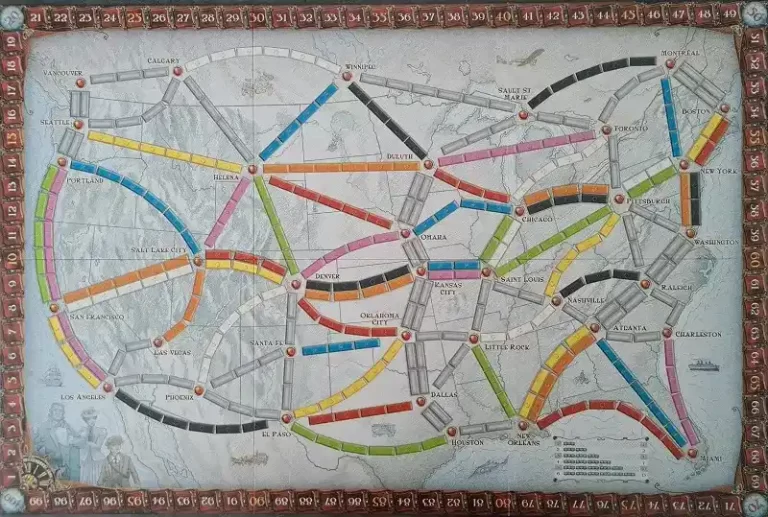
\includegraphics[width=0.8\linewidth]{plateau.png}
\end{frame}

\begin{frame}{Sauvegarde et score}
\textbf{Sauvegarde JSON :}
\begin{itemize}
    \item Sauvegarde/restauration de l'\'etat du jeu
    \item Nom, cartes, routes, joueur actuel
\end{itemize}
\textbf{Calcul de score :}
\begin{itemize}
    \item Routes captur\'ees : points selon longueur
    \item Objectifs : \`a v\'erifier (composantes connexes)
    \item Plus long chemin : \textbf{fonction r\'ecursive} (exploration des routes captur\'ees)
\end{itemize}
\end{frame}

\begin{frame}{Tests unitaires}
\texttt{unittest} + \texttt{patch} pour entr\'ees simul\'ees
\begin{itemize}
    \item Pioche (visible, cach\'ee, locomotive)
    \item Capture de route (succ\`es, cartes insuffisantes, wagons insuffisants)
    \item Objectifs (choix, filtrage)
    \item Sauvegarde (structure JSON)
    \item Bonus plus long chemin
\end{itemize}
\end{frame}

\begin{frame}{Limitations actuelles}
\begin{itemize}
    \item Pas de v\'erification des objectifs atteints (composantes connexes)
    \item Pas encore de joueur intelligent
    \item Interface uniquement graphique (pas interactive)
    \item Probl\`emes de standardisation de couleurs (\"rouge\" vs \"red\")
\end{itemize}
\end{frame}

\begin{frame}{Perspectives et suite}
\textbf{Am\'eliorations pr\'evues :}
\begin{itemize}
    \item Finaliser joueur al\'eatoire puis IA heuristique
    \item Int\'egrer une IHM (Tkinter / PyQt5)
    \item Ajout de tests pour la fin de partie, v\'erif. objectifs
    \item Uniformiser l'affichage et les couleurs
\end{itemize}
\end{frame}

\begin{frame}{Conclusion}
\begin{itemize}
    \item Projet riche, modulable, extensible
    \item Base solide : logique de jeu + affichage + tests
    \item De nombreuses extensions envisageables (IA, IHM, modes de jeu)
    \item Exp\'erience concr\`ete en conception objet, graphe et architecture de projet
\end{itemize}
\end{frame}

\end{document}
